\chapter{Methodology}
\label{cha:methodology}

In order to estimate the theoretical bitcoin mining performance, the performance
of the hashing accelerator is measured both when using a DMA for data transfer
and without a DMA. The results are compared to a software implementation of the
algorithm.

In addition to measuring the hashing performance, the power efficiency of the
solution is evaluated, allowing estimating the number of hashes per W, a number
that can be compared with other hardware.

\section{Test Setup}
\label{sec:SHMAC_setup}

To test the accelerator, a 20~tile setup was used on SHMAC. A 5x4 grid containing the following
tiles were synthesized, resulting in the following setup, also illustrated in figure \ref{fig:5x4}:

\begin{itemize}
    \item 16 CPU tiles with on-tile DMA and SHA256 accelerator
    \item 2 scratchpad tiles
    \item 1 DRAM tile
    \item 1 I/O tile
\end{itemize}

\begin{figure}[ht]
    \centering
    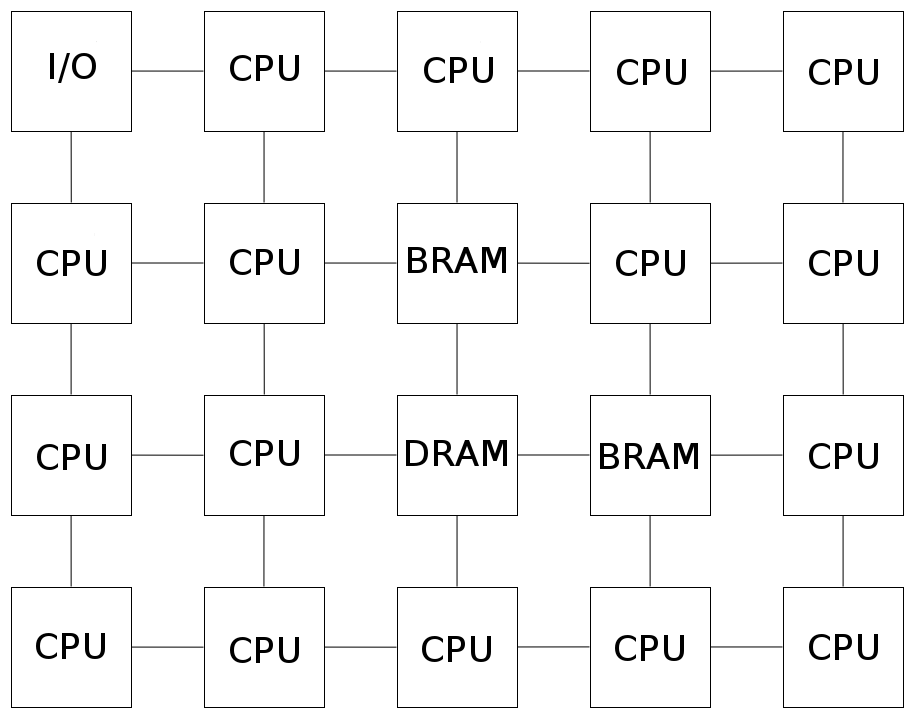
\includegraphics[width=0.5\textwidth]{Figures/Measurements/5x4}
    \caption{Test setup, using BRAM tiles as scratchpad and DRAM as main memory.}
    \label{fig:5x4}
\end{figure}

\section{Measuring the Performance}

Measuring the performance is done by repeatedly double-hashing a block of data, recording the
number of hashes achieved per second per core. By turning on one core at a time, it
is possible to see how the performance scales as more cores are added. Recording
the number of hashes per second per core makes it possible to see how the performance
of each core is affected by the traffic on the network-on-chip generated by the other
cores in the network.

Using the setup described in section \ref{sec:SHMAC_setup}, tests where run using the
following method:

\begin{itemize}
    \item Hashing using software only, not using the SHA256 hashing module or DMA module.
    All work is done by the on-tile processor.
    \item Hashing using only the hashing accelerator.
    The processor controls and copies data to and from the hashing module.
    \item Hashing using the hashing accelerator and DMA.
    The processor controls each module, but the DMA handles data transfer.
\end{itemize}

Interrupts are used by the hashing module to signal when it is finished working. However,
the DMA does not support interrupts and has to be polled while copying data to and from
the module, which may have a minor influence on the results.

\section{Measuring Power Usage}

Power usage for the application is determined by measuring the wall-power of the box
that SHMAC is running on both when idle and when running the test applications. The
power usage of the application is then determined using the following formula, where
$P$ is the power in watts:

\[P_{application} = P_{running} - P_{idle}\]


% NOTE TO SELF: At some point, I think we need to underline the existing problems (cache bug, cache coherency issues, etc.), in order to affirm whenever they affect our test results.
% Furthermore, a report should always provide the means for the results to be reproduced.
% Must discuss with Kristian. - No need, let's add that stuff to the Evaluation chapter.

% FOLLOWING POST-MEETING:

%
%Optional: Write the expected max performance if we can calculate them?
%
%\section{Known hazards with SHMAC}
%List up potential problems that SHMAC may give us, due to the known bugs in the system (cache coherency issues with DMA, the infamous cache bug



